\chapter{The Adjoint in Linear Algebra}

\begin{flushright}
\textit{The adjoint is the same sensitivity question, asked from the other end.}
\end{flushright}

\bigskip

Chapter~4 showed that analytic forward sensitivity analysis for a
model with $m = 50$ parameters requires 50 linear solves, one per
parameter. Each solve uses the same coefficient matrix~$A$, so we
pay once for the LU~factorization and 50~times for back-substitution.
That is still 50~operations.

Now suppose we care about a single response functional, not the
entire solution~$\vec{u}$. The quantity of interest is
$J = \vec{c}^T\vec{u}$: the pollution level at one monitoring station,
the total disease burden, the profit at equilibrium.
We want $\partial J/\partial q$ for all 50~parameters~$q$.

Is there a way to compute all 50~derivatives simultaneously,
in the cost of a \emph{single} linear solve?

Yes. The answer is the adjoint.
The adjoint approach to sensitivity analysis was developed for nonlinear
systems by Cacuci~\cite{cacuci1981sensitivity} and has since become a
standard tool in optimal design and computational science~\cite{giles2000introduction}.

%%------------------------------------------------------------
\section{A Preview: The Same Answer, One Solve Instead of Fifty}
\label{sec:adjoint_preview}
%%------------------------------------------------------------

Before the general theory, work through a small example by hand
to see exactly what the adjoint does and why it is efficient.

\subsection*{The Setup}

Consider the $2 \times 2$ linear system
\begin{equation}
  A\vec{u} = \vec{b}(q_1, q_2),
  \qquad
  A = \begin{pmatrix} 3 & 1 \\ 1 & 2 \end{pmatrix},
  \qquad
  \vec{b} = \begin{pmatrix} q_1 \\ q_2 \end{pmatrix},
  \label{eq:preview_system}
\end{equation}
where $q_1$ and $q_2$ are two parameters of interest.
The scalar response functional is
$J = u_1 + u_2 = \vec{c}^T\vec{u}$ with $\vec{c} = (1,1)^T$.
We want $\partial J/\partial q_1$ and $\partial J/\partial q_2$.

\subsection*{The Direct (Forward) Approach: Two Solves}

Differentiating $A\vec{u} = \vec{b}$ with respect to $q_1$:
$A\,(\partial\vec{u}/\partial q_1) = \partial\vec{b}/\partial q_1 = (1,0)^T$.
Differentiating with respect to $q_2$:
$A\,(\partial\vec{u}/\partial q_2) = \partial\vec{b}/\partial q_2 = (0,1)^T$.
Two linear solves (one per parameter) with the same matrix $A$:

\[
  A^{-1} = \tfrac{1}{5}\begin{pmatrix} 2 & -1 \\ -1 & 3 \end{pmatrix},
  \quad\text{so}\quad
  \pd{\vec{u}}{q_1} = \tfrac{1}{5}\begin{pmatrix}2\\-1\end{pmatrix},
  \qquad
  \pd{\vec{u}}{q_2} = \tfrac{1}{5}\begin{pmatrix}-1\\3\end{pmatrix}.
\]

The derivatives of $J = \vec{c}^T\vec{u}$ are:
\[
  \pd{J}{q_1} = \vec{c}^T\pd{\vec{u}}{q_1}
              = (1,1)\cdot\tfrac{1}{5}(2,-1)^T = \tfrac{1}{5},
  \qquad
  \pd{J}{q_2} = \vec{c}^T\pd{\vec{u}}{q_2}
              = (1,1)\cdot\tfrac{1}{5}(-1,3)^T = \tfrac{2}{5}.
\]
Two solves, two derivatives. For 50 parameters: 50 solves.

\subsection*{The Adjoint Approach: One Solve}

Instead of solving for $\partial\vec{u}/\partial q_j$ separately for each $j$,
introduce the \textbf{adjoint vector} $\vec{v}$ satisfying
\begin{equation}
  A^T\vec{v} = \vec{c}.
  \label{eq:preview_adjoint}
\end{equation}
This is one linear solve with the transposed matrix.
Since $A$ is symmetric here, $A^T = A$, so $\vec{v} = A^{-1}\vec{c}$:
\[
  \vec{v} = A^{-1}\vec{c} = \tfrac{1}{5}\begin{pmatrix}2&-1\\-1&3\end{pmatrix}\begin{pmatrix}1\\1\end{pmatrix}
          = \tfrac{1}{5}\begin{pmatrix}1\\2\end{pmatrix}.
\]

\textbf{What does $\vec{v}$ represent?}
The adjoint vector answers the question: \emph{if the state $\vec{u}$
were perturbed by a small amount $\delta\vec{u}$, how much would $J$ change?}
A direct perturbation gives $\delta J \approx \vec{c}^T\delta\vec{u}$,
but not all $\delta\vec{u}$ are achievable --- the system constraint
$A\vec{u} = \vec{b}$ means only perturbations satisfying
$A\,\delta\vec{u} = \delta\vec{b}$ are reachable.
The adjoint vector $\vec{v}$ encodes how much each component
of the state contributes to $J$, after accounting for
the coupling imposed by the matrix $A$.

In the 2$\times$2 example,
$\vec{v} = \tfrac{1}{5}(1,2)^T$ means that
a perturbation to $u_2$ matters \emph{twice as much}
to $J = u_1 + u_2$ as a perturbation to $u_1$ ---
not because $\vec{c} = (1,1)^T$ treats them equally,
but because the system $A$ couples $u_1$ and $u_2$ differently.
This coupling is what makes the adjoint more than a convenient shortcut:
$\vec{v}$ is the correct sensitivity weighting for the constrained system,
not the naive weighting $\vec{c}$ for the unconstrained response.

Now observe: for any parameter $q_j$,
\[
  \pd{J}{q_j} = \vec{c}^T\pd{\vec{u}}{q_j}
              = (A^T\vec{v})^T\pd{\vec{u}}{q_j}
              = \vec{v}^T\!\underbrace{A\pd{\vec{u}}{q_j}}_{=\,\partial\vec{b}/\partial q_j}
              = \vec{v}^T\pd{\vec{b}}{q_j}.
\]
This is the key step: $A\,(\partial\vec{u}/\partial q_j) = \partial\vec{b}/\partial q_j$
is the FSE right-hand side, a known vector.
No additional solve is needed — just a dot product.

Checking against our direct answers:
\[
  \pd{J}{q_1} = \vec{v}^T\pd{\vec{b}}{q_1}
              = \tfrac{1}{5}(1,2)\cdot(1,0)^T = \tfrac{1}{5} \;\checkmark
  \qquad
  \pd{J}{q_2} = \vec{v}^T\pd{\vec{b}}{q_2}
              = \tfrac{1}{5}(1,2)\cdot(0,1)^T = \tfrac{2}{5} \;\checkmark
\]
One solve for $\vec{v}$, then one dot product per parameter.
For 50 parameters: still one solve, then 50 dot products.
The cost advantage is a factor of 50.

\begin{selfcheck}
Add a third parameter $q_3$ to the system above by setting
$\vec{b} = (q_1 + q_3,\; q_2)^T$. Without solving any new linear
systems, use the adjoint vector $\vec{v}$ already computed
to find $\partial J/\partial q_3$.
\end{selfcheck}
\begin{scAnswer}
$\partial\vec{b}/\partial q_3 = (1,0)^T$.
$\partial J/\partial q_3 = \vec{v}^T(1,0)^T = \frac{1}{5}(1,2)\cdot(1,0)^T = \frac{1}{5}$.
No new solve needed. Adding parameters costs only one dot product each
once $\vec{v}$ is known. This is the computational power of the adjoint.
\end{scAnswer}

\medskip

The pattern above is the entire idea of the adjoint, stripped to its
essentials. Section~\ref{sec:adjoint_strategy} states it precisely.

%%------------------------------------------------------------
\section{The Strategy, Stated Explicitly}
\label{sec:adjoint_strategy}
%%------------------------------------------------------------

The cost analysis above raises the key question: can we recover all $m$ sensitivities without solving $m$ separate systems?
It turns out we can, through a trick that is worth understanding before seeing the symbols.

The adjoint is not a new kind of problem.\index{adjoint method} It is a deliberate trick:
introduce an auxiliary vector, choose it to cancel the unknown
sensitivity variable, and read off the result.
Here is the trick in plain language before any symbols.

\begin{enumerate}[label=\textbf{Step \arabic*.}, leftmargin=2.2cm]

\item We want $\partial J/\partial q_j$ for all parameters $q_j$.
Since $J = \vec{c}^T\vec{u}$, this is
$\partial J/\partial q_j = \vec{c}^T (\partial\vec{u}/\partial q_j)$.
But $\partial\vec{u}/\partial q_j$ requires a separate FSE solve
for every $j$ (50~solves for 50~parameters).

\item Introduce an auxiliary vector $\vec{v}$ and observe that
for any vector $\vec{v}$:
\[
  \vec{c}^T\pd{\vec{u}}{q_j}
  = \vec{v}^T\!\left[A\pd{\vec{u}}{q_j}\right]
    + \left(\vec{c}^T - \vec{v}^T\!A\right)\pd{\vec{u}}{q_j}.
\]
The first term on the right is $\vec{v}^T\vec{r}_j$,
where $\vec{r}_j = A(\partial\vec{u}/\partial q_j)$
is the FSE right-hand side (a known vector once $\vec{u}$ is known).
The second term vanishes if we choose $\vec{v}$ so that $\vec{v}^T A = \vec{c}^T$.

\item Choose $\vec{v}$ to satisfy the \textbf{adjoint equation}:
\begin{equation}
  A^T\vec{v} = \vec{c}.
  \label{eq:adjointeq}
\end{equation}
Then $\vec{c}^T - \vec{v}^T A = \vec{0}$ and the sensitivity formula reduces to:
\begin{equation}
  \pd{J}{q_j} = \vec{v}^T\vec{r}_j
  \qquad\text{for all } j = 1, \ldots, m.
  \label{eq:sensfromula}
\end{equation}
\end{enumerate}

One solve for $\vec{v}$ (equation~\eqref{eq:adjointeq}) recovers
all $m$ sensitivities through formula~\eqref{eq:sensfromula}.
The trick works because the adjoint equation does not depend on $j$:
$\vec{v}$ is determined by $\vec{c}$ and $A$ alone.

The adjoint is not a separate, unrelated problem. It is constructed
entirely from the coefficient matrix $A$ (via transposition)
and the response vector $\vec{c}$ of the forward problem.
Everything about the adjoint is determined by the forward problem.

\begin{selfcheck}
For the system $A\vec{u} = \vec{b}$ with
$A = \begin{pmatrix} 2 & 1 \\ 0 & 3 \end{pmatrix}$
and response functional $J = u_1$ (so $\vec{c} = (1,0)^T$):
write down the adjoint equation~\eqref{eq:adjointeq} and solve for $\vec{v}$.
\end{selfcheck}
\begin{scAnswer}
$A^T\vec{v} = \vec{c}$ becomes
$\begin{pmatrix} 2 & 0 \\ 1 & 3 \end{pmatrix}\vec{v}
= \begin{pmatrix} 1 \\ 0 \end{pmatrix}$.
Solving: $v_1 = 1/2$, $v_2 = -1/6$.
This single solve (one back-substitution with $A^T$) gives us the
sensitivity of $J = u_1$ to any number of parameters,
via formula~\eqref{eq:sensfromula}.
\end{scAnswer}

%%------------------------------------------------------------
\section{The Commutative Diagram}\index{commutative diagram}
\label{sec:commdiagram}
%%------------------------------------------------------------

The three-step strategy and the 2$\times$2 preview both express the same
mathematical fact: the FSE route and the adjoint route reach the same
sensitivity, at different cost.
Figure~\ref{fig:commdiag} shows this as a diagram —
read it as a summary of the algebra already developed,
not as an introduction to the idea.

\begin{figure}[htb]
\centering
\begin{tikzpicture}[
  node distance=2.8cm and 4.8cm,
  box/.style={draw, rounded corners=4pt, minimum width=3.2cm,
              minimum height=1.0cm, align=center, font=\small},
  arr/.style={-{Latex[length=3mm]}, thick},
  darr/.style={-{Latex[length=3mm]}, thick, dashed},
]

%% Nodes
\node[box] (fwd)    {Forward problem\\$A\vec{u} = \vec{b}$};
\node[box, right=of fwd]  (fse)  {FSE\\$A\pd{\vec{u}}{q_j} = \vec{r}_j$};
\node[box, below=of fwd]  (adj)  {Adjoint\\$A^T\vec{v} = \vec{c}$};
\node[box, below=of fse]  (sens) {Sensitivity\\$\pd{J}{q_j}$};

%% Forward path (top, right)
\draw[arr] (fwd) -- node[above, font=\small]{solve for $\vec{u}$} (fse);
\draw[arr] (fse) -- node[right, font=\small]{$\vec{c}^T\pd{\vec{u}}{q_j}$} (sens);

%% Adjoint path (left, bottom)
\draw[darr] (fwd) -- node[left, font=\small]{solve $A^T\vec{v}=\vec{c}$} (adj);
\draw[darr] (adj) -- node[below, font=\small]{$\vec{v}^T\vec{r}_j$} (sens);

%% Labels
\node[font=\small\itshape, above=0.15cm of fse] {Forward path: $m$ solves};
\node[font=\small\itshape, below=0.15cm of adj] {Adjoint path: 1 solve};

\end{tikzpicture}
\caption{The commutative diagram for sensitivity analysis.
         The forward path (solid arrows) computes $\partial J/\partial q_j$
         by solving the FSE for each parameter, $m$~solves total.
         The adjoint path (dashed arrows) solves the adjoint equation
         once, then evaluates the sensitivity formula for each parameter;
         1~solve total.
         Both paths deliver the same result.}
\label{fig:commdiag}
\end{figure}

The diagram commutes: both paths from the forward problem to the
sensitivity give identical results. This can be verified directly
from the algebra in Section~\ref{sec:adjoint_strategy}.

\begin{theorem}[Forward--Adjoint Equivalence]
\label{thm:equiv}
Let $A\vec{u} = \vec{b}$ with $A$ nonsingular, $J = \vec{c}^T\vec{u}$,
and FSE $A\,\partial\vec{u}/\partial q_j = \vec{r}_j$.
Let $\vec{v}$ solve the adjoint equation $A^T\vec{v} = \vec{c}$.
Then
\[
  \pd{J}{q_j} = \vec{c}^T\pd{\vec{u}}{q_j} = \vec{v}^T\vec{r}_j
\]
for every parameter $q_j$.
\end{theorem}

\begin{proof}
$\vec{c}^T(\partial\vec{u}/\partial q_j)
= (A^T\vec{v})^T(\partial\vec{u}/\partial q_j)
= \vec{v}^T A(\partial\vec{u}/\partial q_j)
= \vec{v}^T\vec{r}_j$.
\end{proof}

The adjoint gives \emph{exactly} the same sensitivity values as
the FSE. It is not an approximation. Students sometimes expect that
a method requiring fewer solves must sacrifice accuracy;
here it does not.

\begin{selfcheck}
Using Theorem~\ref{thm:equiv}, state in words why the adjoint
equation does not need to be re-solved when a new parameter $q_k$
is added to the sensitivity study.
\end{selfcheck}
\begin{scAnswer}
The adjoint equation $A^T\vec{v} = \vec{c}$ depends only on
$A$ (the system coefficient matrix) and $\vec{c}$ (the response
vector), neither of which changes when we add a new parameter.
Adding parameter $q_k$ changes only the FSE right-hand side
$\vec{r}_k = \partial\vec{b}/\partial q_k - (\partial A/\partial q_k)\vec{u}$,
which is a known vector once the forward solution $\vec{u}$ is computed.
The sensitivity $\partial J/\partial q_k = \vec{v}^T\vec{r}_k$
is then obtained by a single dot product, no additional linear solve.
\end{scAnswer}

%%------------------------------------------------------------
\section{Cost Comparison and the Decision Rule}
\label{sec:adjcost}
%%------------------------------------------------------------

\subsection{When to Use the Adjoint}

Both the FSE and the adjoint produce the same sensitivity Jacobian.
Their costs differ dramatically when $m$ and $r$ are unequal,
where $m$ is the number of \POIs and $r$ is the number of
response functionals.

For the FSE: one solve per \POI $\to$ $m$~solves total.

For the adjoint: one solve per response functional $\to$ $r$~solves total.

\begin{equation}
  \boxed{m > r \implies \text{use adjoint;} \qquad
         r > m \implies \text{use FSE}.}
  \label{eq:decisionrule}
\end{equation}

In most SA applications, there are many \POIs ($m$ large) and
a small number of \QOIs of primary interest ($r$ small), so
the adjoint is preferred. The canonical situation is $r = 1$:
one scalar response functional (peak infection count, total burden,
profit at equilibrium) and many parameters.

\subsection{Cost Comparison Plot}

Figure~\ref{fig:costcomp} shows the number of linear solves
required by each method as a function of the number of parameters.

\begin{figure}[htb]
\centering
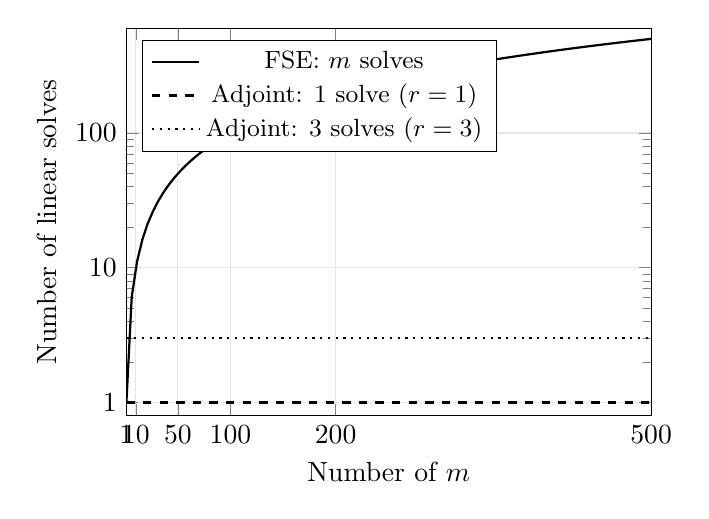
\begin{tikzpicture}
\begin{semilogyaxis}[
  width=0.68\textwidth, height=6.5cm,
  xlabel={Number of \POIs $m$},
  ylabel={Number of linear solves},
  xmin=1, xmax=500,
  ymin=0.8, ymax=600,
  xtick={1,10,50,100,200,500},
  ytick={1,10,100},
  yticklabels={1,10,100},
  grid=major, grid style={gray!20},
  legend pos=north west,
  legend style={font=\small},
]
\addplot[thick, black, domain=1:500, samples=100] {x};
  \addlegendentry{FSE: $m$ solves}
\addplot[thick, dashed, black] coordinates {(1,1)(500,1)};
  \addlegendentry{Adjoint: 1 solve ($r=1$)}
\addplot[thick, dotted, black] coordinates {(1,3)(500,3)};
  \addlegendentry{Adjoint: 3 solves ($r=3$)}
\end{semilogyaxis}
\end{tikzpicture}
\caption{Cost comparison for FSE vs.\ adjoint sensitivity analysis,
         measured in number of linear solves.
         For $r = 1$ response functional (dashed), the adjoint
         always requires exactly 1~solve regardless of $m$.
         For $r = 3$ (dotted), the adjoint requires 3~solves.
         The FSE requires $m$~solves.
         The crossover occurs at $m = r$; for $m > r$, the adjoint wins.}
\label{fig:costcomp}
\end{figure}

For the symbiotic population model ($m = 3$ parameters,
$r = 2$ response functionals $\{\bar{u}_1, \bar{u}_2\}$):
FSE requires 3~solves; adjoint requires 2.
The advantage is modest here.
For the malaria model ($m = 17$, $r = 1$): FSE requires 17~solves;
adjoint requires 1.
For a climate model ($m = 200$, $r = 2$): FSE requires 200~solves;
adjoint requires 2: a factor of 100~improvement.

\begin{selfcheck}
A model has $m = 30$ \POIs and $r = 5$ response functionals.
Each linear solve takes 2~minutes.
How long does the FSE approach take?
How long does the adjoint approach take?
At what value of $r$ would the two approaches have equal cost?
\end{selfcheck}
\begin{scAnswer}
FSE: $30 \times 2 = 60$~minutes.
Adjoint: $5 \times 2 = 10$~minutes. Savings: 50~minutes.
Equal cost when $r = m = 30$.
\end{scAnswer}

%%------------------------------------------------------------
\section{The Symbiotic Population: Full Adjoint Treatment}
\label{sec:sympAdj}
%%------------------------------------------------------------

We now apply the adjoint to the symbiotic population equilibrium
from Chapter~4, comparing the forward and adjoint approaches
side by side. The forward problem is $A\vec{\bar{u}} = \vec{b}$
at equilibrium, with $A = D_{\vec{u}}[\vec{f}]$ as in
equation~(4.7). The comparison makes the cost advantage concrete.

\subsection{FSE Approach: Three Parameters, Three Solves}

For parameters $a$, $b$, $c$, the FSE requires solving
$A(\partial\vec{\bar{u}}/\partial q_j) = -\partial\vec{f}/\partial q_j$
for $j = a, b, c$, three linear solves with the same matrix $A$,
one LU factorization and three back-substitutions.

\subsection{Adjoint Approach: Two Solves for Two Response Functionals}

Now suppose we want $\partial J_1/\partial q_j$ and
$\partial J_2/\partial q_j$ for all three parameters,
where $J_1 = \bar{u}_1$ and $J_2 = \bar{u}_2$.
The response vectors are $\vec{c}_1 = (1,0)^T$ and
$\vec{c}_2 = (0,1)^T$.

The two adjoint equations are:
\begin{equation}
  A^T\vec{v}_1 = \vec{c}_1 = \begin{pmatrix}1\\0\end{pmatrix},
  \qquad
  A^T\vec{v}_2 = \vec{c}_2 = \begin{pmatrix}0\\1\end{pmatrix}.
  \label{eq:sympAdjEqs}
\end{equation}
Two solves (one per response functional) give $\vec{v}_1$ and $\vec{v}_2$.

\medskip\noindent
\textbf{A note on correlated QOIs.}
Even when the \POIs are independent (uncorrelated inputs),
the \QOIs are almost always correlated outputs:
$J_1 = \bar{u}_1$ and $J_2 = \bar{u}_2$ both depend on the same
equilibrium $\vec{\bar{u}}$, so perturbations to any parameter
affect both simultaneously.
This is not a problem for the adjoint method; it is simply a property
of the model.
The adjoint computes each $\partial J_k / \partial q_j$ independently
by solving $A^T\vec{v}_k = \vec{c}_k$ for each response functional.
Any statistical correlation among the $J_k$'s is a property of the model,
not an issue for the adjoint method --- no special handling is required.
The adjoint naturally produces correct, consistent sensitivities
for all $r$ response functionals by virtue of operating through
the same forward solution $\vec{\bar{u}}$.

The sensitivities follow from formula~\eqref{eq:sensfromula}:
\begin{equation}
  \pd{J_k}{q_j} = \vec{v}_k^T\vec{r}_j,
  \qquad
  \vec{r}_j = -\pd{\vec{f}}{q_j},
  \label{eq:sympSens}
\end{equation}
giving all $2 \times 3 = 6$ sensitivities from two adjoint solves
rather than three FSE solves.

\subsection{Verification}

Theorem~\ref{thm:equiv} guarantees the two approaches give identical
results. At nominal values $a = 0.4$, $b = 1$, $c = 0.3$:
\begin{center}
\renewcommand{\arraystretch}{1.3}
\begin{tabular}{lcccccc}
\toprule
 & $\SI{a}{\bar{u}_1}$ & $\SI{b}{\bar{u}_1}$ & $\SI{c}{\bar{u}_1}$
 & $\SI{a}{\bar{u}_2}$ & $\SI{b}{\bar{u}_2}$ & $\SI{c}{\bar{u}_2}$ \\
\midrule
FSE (3 solves)    & $-0.530$ & $0$ & $0.136$ & $+0.136$ & $0$ & $-0.292$ \\
Adjoint (2 solves)& $-0.530$ & $0$ & $0.136$ & $+0.136$ & $0$ & $-0.292$ \\
\bottomrule
\end{tabular}
\end{center}

The rows are identical. The adjoint is not an approximation.

\medskip

A structural observation: the two adjoint solutions
$\vec{v}_1, \vec{v}_2$ are the columns of $(A^T)^{-1}$,
which equals $(A^{-1})^T$. Collecting all adjoint solutions
into a matrix therefore gives the transpose of the inverse.
This connection is intellectually interesting but not computationally useful:
we never form $A^{-1}$ explicitly, we extract the product
$\vec{v}_k^T\vec{r}_j$ for each required sensitivity, which is
far cheaper than computing the full inverse matrix.

%%------------------------------------------------------------
\section{Reverse Mode and Backpropagation}
\label{sec:reversemodeAD}
%%------------------------------------------------------------

The adjoint strategy of the preceding sections applies to
linear systems. This section extends it to arbitrary differentiable
computations via the computation graph, revealing the connection
to algorithmic differentiation and, through it, to the training
of neural networks.

\subsection{The Computation Graph}

Every differentiable computation can be represented as a directed
acyclic graph in which each node holds an intermediate value
and each edge represents an elementary operation (addition,
multiplication, division, elementary function).

For $R_0 = k\beta/\gamma$, the computation graph is:
\begin{equation}
  k, \beta \xrightarrow{\times} v_1 = k\beta
  \xrightarrow{\div\gamma} v_2 = k\beta/\gamma = R_0.
  \label{eq:R0graph}
\end{equation}
Reading left to right is the forward evaluation:
given $k$, $\beta$, $\gamma$, compute $R_0$.

\subsection{Forward Mode: One Pass Per Input}

In \textbf{forward mode}\index{algorithmic differentiation!forward mode} differentiation, we propagate derivatives
$\dot{v}_i = \partial v_i/\partial q$ through the graph
for one input $q$ at a time.

For $q = k$: set $\dot{k} = 1$, $\dot{\beta} = 0$, $\dot{\gamma} = 0$.
Propagate forward:
\[
  \dot{v}_1 = \dot{k}\beta + k\dot{\beta} = \beta,
  \qquad
  \dot{R}_0 = \dot{v}_1/\gamma - v_1\dot{\gamma}/\gamma^2 = \beta/\gamma.
\]
So $\partial R_0/\partial k = \beta/\gamma$.
Repeat with $\dot{\beta} = 1$ to get $\partial R_0/\partial\beta$.
Repeat with $\dot{\gamma} = 1$ to get $\partial R_0/\partial\gamma$.
Total: 3~forward passes for 3~parameters.

\subsection{Reverse Mode: One Pass for All Inputs}

In \textbf{reverse mode}\index{algorithmic differentiation!reverse mode} differentiation, we propagate the adjoint
variable $\bar{v}_i = \partial J/\partial v_i$ backward through
the graph.

Set $\bar{R}_0 = \partial J/\partial R_0 = 1$ (we are computing
$\partial R_0/\partial(\cdot)$, so $J = R_0$).
Propagate backward:
\begin{align}
  \bar{v}_1   &= \bar{R}_0 \cdot \pd{R_0}{v_1} = 1 \cdot (1/\gamma) = 1/\gamma,
               \label{eq:rev1}\\
  \bar{k}     &= \bar{v}_1 \cdot \pd{v_1}{k}   = (1/\gamma)\cdot\beta = \beta/\gamma,
               \label{eq:rev2}\\
  \bar{\beta}  &= \bar{v}_1 \cdot \pd{v_1}{\beta} = (1/\gamma)\cdot k = k/\gamma,
               \label{eq:rev3}\\
  \bar{\gamma} &= \bar{R}_0 \cdot \pd{R_0}{\gamma} = 1\cdot(-v_1/\gamma^2)
                = -k\beta/\gamma^2.
               \label{eq:rev4}
\end{align}
One backward pass gives all three derivatives simultaneously:
\[
  \pd{R_0}{k} = \bar{k} = \frac{\beta}{\gamma}, \quad
  \pd{R_0}{\beta} = \bar{\beta} = \frac{k}{\gamma}, \quad
  \pd{R_0}{\gamma} = \bar{\gamma} = -\frac{k\beta}{\gamma^2}.
\]
These match the analytic results. The reverse pass cost is
proportional to the graph size, one pass regardless of the
number of inputs.

Table~\ref{tab:fwdrev} summarizes the comparison.

\begin{table}[htb]
\centering
\begin{tabular}{lll}
\toprule
 & Forward mode & Reverse mode \\
\midrule
Propagates       & $\dot{v}_i = \partial v_i/\partial q$ (one $q$) &
                   $\bar{v}_i = \partial J/\partial v_i$ (one $J$) \\
Direction        & Input $\to$ output & Output $\to$ input \\
Cost             & 1 pass per input & 1 pass per output \\
Preferred when   & $m \leq r$ (few inputs) & $m \geq r$ (few outputs) \\
Matrix analog    & FSE: $A\,\partial\vec{u}/\partial q_j = \vec{r}_j$ &
                   Adjoint: $A^T\vec{v} = \vec{c}$ \\
\bottomrule
\end{tabular}
\caption{Forward mode and reverse mode differentiation:
         a side-by-side comparison.
         The matrix analogs confirm that the two modes are
         the computation-graph generalizations of the FSE and
         adjoint approaches from Sections~\ref{sec:adjoint_strategy}--\ref{sec:adjcost}.}
\label{tab:fwdrev}
\end{table}

\subsection{The Backpropagation Connection\index{backpropagation}}

\medskip\noindent
\textit{Note for readers without machine learning background:
this subsection connects the adjoint to neural network training.
If backpropagation is unfamiliar, skip this subsection and proceed
to Chapter~6 --- the adjoint ODE does not depend on it.
Return here after completing Chapter~6 if you want the connection.}

\medskip

If you have encountered training a neural network, you have already
used the adjoint under a different name.

A neural network is a composition of parameterized functions.
Training minimizes a loss function $J(\theta)$ over parameters
$\theta$ using gradient descent, which requires $\partial J/\partial\theta_i$
for every parameter~$\theta_i$.
The loss function is a scalar ($r = 1$) and modern networks have
millions of parameters ($m \gg 1$), so reverse mode is overwhelmingly
preferred. Backpropagation is exactly the reverse-mode computation
described above, applied to the computation graph of the network.

To map notation explicitly: each computation-graph node $v_i$ corresponds
to the $i$-th standard basis vector $\vec{e}_i$, and the adjoint variable
$\lambda_i = \partial J/\partial v_i$ records how much $J$ changes per unit
change at node $i$ --- exactly the role played by $\bar{v}_i$ in reverse mode.

The adjoint equation for the ODE case, derived in Chapter~6,
is the continuous limit of this discrete backward accumulation.
The backward ODE for $\lambda(t)$ is the functional-analytic
version of the backward pass through the computation graph.

\unifyingidea{2} The adjoint is the transpose in whatever space
you are working in.

In this chapter: the adjoint equation is $A^T\vec{v} = \vec{c}$,
the transposed coefficient matrix applied to the adjoint vector.

In the computation graph: reverse mode is the chain rule applied
in reverse order, accumulating $\bar{v}_i = \partial J/\partial v_i$
backward through the graph.

In Chapter~6: the adjoint will be an ODE running backward in time,
with a terminal condition at $t = T$.
The integration-by-parts identity that produces this ODE is the
functional-analytic analog of the matrix transposition that produced
$A^T$ here.

One idea. Three settings. One cost advantage: when $m \gg r$,
the adjoint/reverse-mode is the preferred computational strategy.

\begin{selfcheck}
Use the reverse-mode computation of equations~\eqref{eq:rev1}--\eqref{eq:rev4}
to compute $\SI{k}{R_0}$, $\SI{\beta}{R_0}$, and $\SI{\gamma}{R_0}$.
Express each as a pure number and verify using the Chapter~2 results.
\end{selfcheck}
\begin{scAnswer}
$\partial R_0/\partial k = \beta/\gamma$.
$\SI{k}{R_0} = (k/R_0)(\partial R_0/\partial k)
= (k/(k\beta/\gamma))\cdot(\beta/\gamma) = 1$.

$\partial R_0/\partial\beta = k/\gamma$.
$\SI{\beta}{R_0} = (\beta/(k\beta/\gamma))(k/\gamma) = 1$.

$\partial R_0/\partial\gamma = -k\beta/\gamma^2$.
$\SI{\gamma}{R_0} = (\gamma/(k\beta/\gamma))(-k\beta/\gamma^2) = -1$.

All three match the Chapter~2 results. The reverse-mode computation
recovers the full sensitivity Jacobian in one pass.
\end{scAnswer}

%%------------------------------------------------------------
\section{Bridge to Chapter 6}
\label{sec:bridge}
%%------------------------------------------------------------

Students sometimes expect the adjoint for differential equations
to require advanced functional analysis (Hilbert spaces,
adjoint operators, and formal operator theory.
Appendix~\ref{app:innerproduct} provides the $L^2$ inner product and
orthogonality needed for that formalism; Appendix~\ref{app:adjointformalism}
develops the full abstract operator framework that makes the connection rigorous.
The preceding sections show why this expectation is misplaced:
the core idea is the matrix transpose.
Every formal construct in Chapter~6 is the natural extension
of the matrix algebra developed here.
Reading Chapter~6 with this chapter in mind, the abstract
notation should feel like familiar territory.

\unifyingidea{1} Every sensitivity value computed in
Section~\ref{sec:sympAdj}, via the adjoint, is a normalized
derivative, an instance of Unifying Idea~1 from Chapter~1.
The adjoint is a computational strategy; the quantity it produces
is still the SI defined in Chapter~2.
The two commutative paths in Figure~\ref{fig:commdiag} produce
the same sensitivity index by different routes.

Chapter~5 has established the adjoint for linear systems.
Chapter~6 extends every result to ordinary differential equations.
The sensitivity Jacobian computed in this chapter is the same object
that Smith~\cite{smith2014uncertainty} uses in \S6.1 to drive
parameter selection and optimal experimental design; students who
complete Chapter~6 will find \S6.1 of Smith immediately accessible.

The translation is direct:

\begin{center}
\renewcommand{\arraystretch}{1.5}
\begin{tabular}{ll}
\toprule
Chapter~5 (linear algebra) & Chapter~6 (dynamical systems) \\
\midrule
Coefficient matrix $A$ & Differential operator $d/dt - J(t)$ \\
Transpose $A^T$ & Adjoint operator $-(d/dt + J(t)^T)$ \\
Adjoint equation $A^T\vec{v} = \vec{c}$ &
  Adjoint ODE $-\dot{\lambda} = J^T\lambda + g_u$ \\
Terminal condition: none & Terminal condition: $\lambda(T) = h_u^T$ \\
Sensitivity formula $\vec{v}^T\vec{r}_j$ &
  Sensitivity formula $\int_0^T\lambda^T F_{p_j}\,dt$ \\
Cost: 1 solve for any $m$ & Cost: 2 ODE solves for any $m$ \\
\bottomrule
\end{tabular}
\end{center}

The integration-by-parts identity in Chapter~6 plays the role of
the algebraic transposition here. The terminal condition on $\lambda(T)$
is the time-dependent analog of the right-hand side $\vec{c}$ in
$A^T\vec{v} = \vec{c}$. The cost advantage is identical: one solve
(or two, for the ODE case where a forward solve is also needed)
recovers all $m$ sensitivities regardless of $m$.

\medskip
In Chapter~6 we extend every result of this chapter to ordinary
differential equations.
The matrix $A$ becomes a differential operator.
The transpose $A^T$ becomes the adjoint differential operator.
The linear solve $A^T\vec{v} = \vec{c}$ becomes an ODE for
$\lambda(t)$ with a terminal condition at $t = T$.
The sensitivity formula $\vec{v}^T\vec{r}_j$ becomes an integral
over $[0,T]$.
The cost advantage is the same: 2~ODE solves instead of $m$.
\medskip

%%------------------------------------------------------------
\section{MATLAB Laboratory: Forward vs.\ Adjoint}
\label{sec:ch5matlab}
%%------------------------------------------------------------

This laboratory compares the FSE and adjoint computations on the
symbiotic population model, then implements reverse-mode
differentiation for $R_0$.

\textbf{Part 1: Symbiotic population via FSE.}
At nominal values $a = 0.4$, $b = 1$, $c = 0.3$, compute
the equilibrium using equation~(4.6). Assemble the Jacobian~$A$
and compute the LU factorization using MATLAB's \texttt{lu}.
Solve the three FSEs ($\partial\vec{\bar{u}}/\partial a$,
$\partial\vec{\bar{u}}/\partial b$, $\partial\vec{\bar{u}}/\partial c$)
using \texttt{U\textbackslash(L\textbackslash r)} for each.
Record the time.

\textbf{Part 2: Symbiotic population via adjoint.}
Solve the two adjoint equations $A^T\vec{v}_1 = \vec{c}_1$ and
$A^T\vec{v}_2 = \vec{c}_2$ using the same LU factorization (with
transposed triangular solves). Compute all 6~sensitivities via
$\vec{v}_k^T\vec{r}_j$. Record the time and verify that all 6~values
agree with Part~1 to machine precision.

\medskip\noindent
\textit{MATLAB note on the transposed solve.}
MATLAB's \texttt{lu} gives $A = P^T L U$, so $A^T = U^T L^T P$.
Solving $A^T\vec{v} = \vec{c}$ therefore proceeds in three steps:
$U^T\vec{w}_1 = P\vec{c}$, then $L^T\vec{w}_2 = \vec{w}_1$, then $\vec{v} = \vec{w}_2$.
In MATLAB this is written compactly as \texttt{L' \textbackslash\ (U' \textbackslash\ (P'*c))},
reading right to left: first multiply by \texttt{P'}, then solve the two
transposed triangular systems.

\begin{verbatim}
%% Assemble Jacobian at equilibrium (see Chapter 4)
A = jac_symp(ubar, a, b, c);
[L, U, P] = lu(A);

%% FSE: 3 solves
for j = 1:3
    rj = rhs_symp(ubar, j);          %% FSE right-hand side
    dwdp(:,j) = U \ (L \ (P * rj));
end

%% Adjoint: 2 solves
c1 = [1;0]; c2 = [0;1];
v1 = L' \ (U' \ (P' * c1));   %% solve A^T v1 = c1
v2 = L' \ (U' \ (P' * c2));   %% solve A^T v2 = c2
for j = 1:3
    rj = rhs_symp(ubar, j);
    dJdp(1,j) = v1' * rj;     %% dJ1/dp_j
    dJdp(2,j) = v2' * rj;     %% dJ2/dp_j
end
\end{verbatim}

\textbf{Part 3: Timing as a function of system size.}
For random systems of size $n = 5, 10, 50, 100$ with $m = 20$
parameters and $r = 1$ response functional, time both approaches.
Plot computation time vs.\ $n$ on log-log axes.
Does the ratio of times approach $m/r = 20$ as expected?

\textbf{Part 4: Reverse-mode $R_0$ by hand.}
Implement the reverse-mode computation~\eqref{eq:rev1}--\eqref{eq:rev4}
in MATLAB for $R_0 = k\beta/\gamma$.
Verify all three sensitivities against the MATLAB Symbolic Toolbox.
Count the number of arithmetic operations in forward mode
vs.\ reverse mode for this graph.

\textbf{Part 5: Verify that adjoint = 50 FSE solves.}
Set up a random $10\times10$ system with $m = 50$ parameters and $r = 1$.
Compute $\partial J/\partial q_j$ for all $j$ by:
(a) 50~FSE solves (forward path); (b) 1~adjoint solve (adjoint path).
Verify that the maximum absolute difference is less than $10^{-12}$.

%%------------------------------------------------------------
\section{Exercises}
%%------------------------------------------------------------

\begin{exercise}[\bloom{L2}]
\label{ex:ch5:strategy}
State the three-step adjoint strategy from Section~\ref{sec:adjoint_strategy}
in your own words, using no symbols.
Then explain: why does the adjoint equation $A^T\vec{v} = \vec{c}$ not
depend on which parameter $q_j$ we are differentiating with respect to?
Why does this independence make the adjoint efficient?
\end{exercise}

\begin{exercise}[\bloom{L3}]
\label{ex:ch5:2x2}
For the linear system
\[
  A\vec{u} = \vec{b}, \qquad
  A = \begin{pmatrix} 3 & 1 \\ 1 & 2 \end{pmatrix}, \quad
  \vec{b} = \begin{pmatrix} b_1(q) \\ b_2(q) \end{pmatrix}
  = \begin{pmatrix} q \\ 2q \end{pmatrix},
\]
with response functional $J = u_1 + u_2$ (so $\vec{c} = (1,1)^T$):
\begin{enumerate}[label=(\alph*)]
  \item Solve the forward problem to find $\vec{u}(q)$ at $q = 1$.
  \item Write and solve the FSE for $\partial\vec{u}/\partial q$.
  \item Write and solve the adjoint equation.
  \item Use formula~\eqref{eq:sensfromula} to compute $\partial J/\partial q$.
  \item Verify by differentiating $J(q) = u_1(q) + u_2(q)$ directly.
\end{enumerate}
\end{exercise}

\begin{exercise}[\bloom{L3}]
\label{ex:ch5:decisionrule}
For each scenario below, state whether you would use the FSE or the adjoint,
and calculate the number of linear solves each approach requires.
\begin{enumerate}[label=(\alph*)]
  \item $m = 5$ parameters, $r = 20$ response functionals.
  \item $m = 100$ parameters, $r = 3$ response functionals.
  \item $m = 8$ parameters, $r = 8$ response functionals.
  \item $m = 1{,}000$ parameters, $r = 1$ response functional.
        Each solve takes 0.1~seconds. How much faster is the preferred method?
\end{enumerate}
\end{exercise}

\begin{exercise}[\bloom{L4}]
\label{ex:ch5:symbiotic}
For the symbiotic population equilibrium with parameters
$a = 0.5$, $b = 2$, $c = 0.4$:
\begin{enumerate}[label=(\alph*)]
  \item Compute all 6~sensitivities ($\SI{a}{\bar{u}_1}$,
        $\SI{b}{\bar{u}_1}$, $\SI{c}{\bar{u}_1}$,
        $\SI{a}{\bar{u}_2}$, $\SI{b}{\bar{u}_2}$, $\SI{c}{\bar{u}_2}$)
        using the FSE approach (3 solves).
  \item Compute the same 6~sensitivities using the adjoint approach (2 solves).
  \item Verify that the two methods agree.
  \item Which approach requires fewer solves? By how much?
        At what values of $m$ and $r$ would the FSE be preferred?
\end{enumerate}
\end{exercise}

\begin{exercise}[\bloom{L4}]
\label{ex:ch5:reverseSEIR}
The SEIR basic reproduction number is
$R_0 = k\beta\nu/[(\nu+\mu)(\gamma+\mu)]$
with parameters $k$, $\beta$, $\nu$ (exposure rate), $\gamma$ (recovery rate),
$\mu$ (mortality rate).
\begin{enumerate}[label=(\alph*)]
  \item Draw the computation graph for $R_0$ (intermediate nodes and edges).
  \item Implement the forward-mode computation to find $\partial R_0/\partial\nu$.
        Count the number of arithmetic operations.
  \item Implement the reverse-mode computation to find all five
        derivatives $\partial R_0/\partial k$, $\partial R_0/\partial\beta$,
        $\partial R_0/\partial\nu$, $\partial R_0/\partial\gamma$,
        $\partial R_0/\partial\mu$ in one backward pass.
  \item Compute the five normalized sensitivity indices and produce a
        tornado plot using interpretable \POIs (mean times, not rates).
\end{enumerate}
\end{exercise}

\begin{exercise}[\bloom{L5}]
\label{ex:ch5:design}
A water-quality model of a river system has $m = 40$ parameters
(pollution source rates, degradation rates, flow speeds, mixing coefficients)
and $r = 2$ response functionals: (1) pollutant concentration at a
downstream monitoring station, and (2) total pollutant load entering
a protected estuary.

Design a complete SA study using the adjoint method.
Specify:
\begin{enumerate}[label=(\alph*)]
  \item The form of the adjoint equation for this model.
  \item How many adjoint solves are required and why.
  \item How you would validate the implementation.
  \item How you would use the sensitivity results to advise
        regulators on which pollution sources to prioritize.
  \item One situation where the adjoint results might be misleading,
        and what you would do to detect and correct it.
\end{enumerate}
\end{exercise}

\begin{exercise}[\bloom{L6}]
\label{ex:ch5:critique}
A colleague states: ``The adjoint always gives the same answer as
forward SA, just faster. So if we already have the FSE code working,
there is no reason to implement the adjoint.''

Evaluate this claim carefully.
\begin{enumerate}[label=(\alph*)]
  \item Is the first sentence (same answer, just faster) correct?
        Give a precise mathematical justification.
  \item Is the second sentence (no reason to implement the adjoint)
        correct? Describe at least two situations where switching from
        FSE to adjoint would be strongly advisable.
  \item For the FSE to be preferred over the adjoint, what relationship
        between $m$ and $r$ must hold? Give a specific numerical example
        where FSE is strictly better.
\end{enumerate}
\end{exercise}

%%------------------------------------------------------------

